\documentclass[british,titlepage]{ntnuthesis}
\usepackage{todonotes}
\usepackage{siunitx}
\usepackage{hhline}
\usepackage{bm}
\usepackage{multirow}
\usepackage{import}

\DeclareSIUnit{\molar}{M}

\emergencystretch=1em % Avoids overfull bibliography

\title{X-ray Computed Tomography Denoising with Generative Adversarial Networks}
% \title{X-ray Computed Tomography Denoising with Generative Adversarial Networks}
\shorttitle{X-ray CT Denoising with GAN}
\author{Trygve Scheline Urdahl}
\shortauthor{T.S. Urdahl}
\date{\today}

\addbibresource{thesis.bib}


% Update glossaries (in terminal):
% pdflatex thesis.tex
% makeglossaries thesis
% pdflatex thesis.tex

% From https://www.overleaf.com/learn/latex/Glossaries

\makeglossaries % Prepare for adding glossary entries


\newglossaryentry{latex}
{
        name=latex,
        description={Is a mark up language specially suited for
scientific documents}
}

\newglossaryentry{bibliography}
{
        name=bibliography,
        plural=bibliographies,
        description={A list of the books referred to in a scholarly work,
typically printed as an appendix}
}

\newglossaryentry{maths}
{
    name=mathematics,
    description={Mathematics is what mathematicians do}
}


% --------------------
% ----- Acronyms -----
% --------------------

\newacronym[\glslongpluralkey={Generative Adversarial Networks}]{gan}{GAN}{Generative Adversarial Network}
\newacronym{cnn}{CNN}{Convolutional Neural Network}
\newacronym{ann}{ANN}{Artificial Neural Network}
\newacronym{ml}{ML}{Machine Learning}
\newacronym{ai}{AI}{Artificial Intelligence}

\newacronym{ct}{CT}{Computed Tomography}
\newacronym{fbp}{FBP}{Filtered Back Projection} % add glossary and acronym lists before document

\begin{document}

\chapter*{Abstract}
X-ray computed tomography (CT) allows for non-destructive imaging of internal structures of materials. The process of creating CT images involves recording x-ray projections of a sample, and computationally reconstructing the projections into a 3D image of the sample. There is an increasing need to extend the methodology to imaging dynamical processes and also limit radiation induced damage on the studied materials. This requires that the projections are obtained with very little capture time and/or the number of projections are reduced. Such data collection strategies will result in noisy and artifact prone reconstructed images. In this thesis we utilize \textit{generative adversarial networks} (GANs), a form of machine learning model, to denoise subsampled and noisy CT images. 

A GAN has been trained to map noisy CT images to high-quality CT images, effectively denoising them. The GAN improves the structural similarity index measure (SSIM) of the noisy reconstruction from $0.233$ to $0.789$, and the mean squared error from $704.4$ to $210.8$, when denoising an undersampled CT dataset containing $46$ uniformly sampled projections from a high-quality dataset which contains $1500$ projections. The GAN has been tested for a range of undersampling levels as well as modifying the loss function. A log-cosh term has been introduced to the loss function used to train the GAN, yielding an improvement in the achieved SSIM from $0.788$ to $0.789$ for the aforementioned undersampled reconstruction, without introducing any discernible drawbacks. 

The GAN denoising has been compared to a \textit{prior image constrained compressed sensing} (PICCS) reconstruction of a dynamic CT dataset. The GAN denoising achieves comparable image quality to the PICCS reconstruction, with some sample details not distinguishable in the PICCS reconstruction being captured by the GAN denoised reconstruction. 

Interaxial banding artifacts are introduced when denoising 2D slices of a 3D sample along an axial plane. These artifacts are reduced by using a depth parameter when training the GAN, allowing the denoising to utilize 3D spatial information from adjacent slices. 
\chapter*{Sammendrag}

\tableofcontents
\listoffigures
\listoftables
% \lstlistoflistings % NB: Caused paragraph indents to disappear, changed the .cls file at bottom. Commented out some lines. 

\printglossary[type=\acronymtype,nonumberlist,style=super] % Print acronyms nogroupskip
%\printglossary                    % Print glossary
% \addcontentsline{toc}{chapter}{Acronyms} % Should not be needed?

\chapter{Introduction}
\label{sec:introduction}

\acrfull{gan} \cite{goodfellow2014gan,goodfellow2020gan}
\todo[inline]{}

\section{Motivation}

\section{Goal of Work}

\section{Thesis Structure}
\chapter{X-Ray Computed Tomography}
\label{sec:ct}
While this thesis is primarily focused on noise reduction using \acrshort{gan}s, a brief overview of some of the basic principles behind \acrfull{ct} imaging will be given in this chapter. The focus will be on explaining the underlying theoretical foundation of \acrshort{ct} imaging, including the main sources of noise. An overview of common reconstruction methods, as well a more novel one, will also be presented.

\section{Theoretical Foundation}
\label{sec:ct:theoreticalfoundation}
X-ray \acrshort{ct} imaging is based on interaction between X-rays and matter. This interaction will attenuate X-rays that propagate through a sample according to the Beer-Lambert law, which is given as \cite{doi:10.1063/1.4950807}
\begin{equation}
    \label{eq:beerlambert}
    I = I_0 \rm{e}^{-\int_{l_0}^{l}\mu\left(x,y,E\right)dl},
\end{equation}
where $I_0$ and $I$ are the incident and the attenuated X-ray beam intensities at positions $l_0$ and $l$ respectively, and $\mu$ is the attenuation coefficient of the traversed matter. The integral in the exponent is the path of the beam through the sample. The attenuation coefficient is dependent on energy ($E$), and typical X-ray \acrshort{ct} systems span a range of wavelengths (i.e. energies). 
Because of this, \cref{eq:beerlambert} must be modified to also account for the polychromatic nature of the X-ray source. 

The total incident radiation can be determined by integrating over all photon energies, 
\begin{equation}
    \label{eq:incidentradiation}
    I_0 = \int_{E_{min}}^{E_{max}}N\left(V,I\right)S\left(E\right)D\left(E\right)dE,
\end{equation}
with $N\left(V,I\right)$ being a variable introduced to account for photon flux depending on X-ray source tube voltage $V$ and current $I$, $S\left(E\right)$ being the normalized X-ray source spectrum modulated by the absorption materials between the source and the detector (not including the sample), and $D\left(E\right)$ being the detector sensitivity modulated by protection materials on the detector. $E_{min}$ and $E_{max}$ bound the energy range of the radiation spectrum. 

By combining \cref{eq:beerlambert,eq:incidentradiation}, we get the modified Beer-Lambert law accounting for the polychromatic X-rays \cite{doi:10.1063/1.4950807}, 
\begin{equation}
    I = \int_{E_{min}}^{E_{max}}N\left(V,I\right)S\left(E\right)D\left(E\right)\rm{e}^{-\int_{l_0}^{l}\mu\left(x,y,E\right)dl}dE.
\end{equation}
This can be solved for the attenuation coefficient projection, giving \cite{doi:10.1063/1.4950807}
\begin{equation}
    \label{eq:ctattenuationcoefficient}
    \int_{l_0}^{l} \mu_m\left(x,y\right)dl = -\ln\left[\frac{\int S\left(E\right) D\left(E\right)\rm{e}^{-\int_{l_0}^{l}\mu\left(x,y,E\right)dl} dE }{ \int S\left(E\right) D\left(E\right) dE }\right].
\end{equation}
The attenuated intensity $I$ can be related to the attenuation coefficient projection $\mu_m$ of a path through the sample by use of this equation. When the attenuation coefficient projections are known, the sample itself can be reconstructed using a reconstruction algorithm if a sufficient number of projections are available. 

\subsection{Noise}
Assuming a sufficient number of projections of the attenuation coefficient are available, the primary sources of noise in \acrshort{ct} measurements are quantum noise and electronic noise \cite{boas2012ct}. 

The quantum noise, sometimes also known as shot noise or simply Poisson noise, is due to the statistical error of low photon counts. It can be modeled as a Poisson distribution \cite{Whiting2006},
\begin{equation}
    \label{eq:poissonnoise}
    P(X = x) = \frac{\rm{e}^{-xm}m^x}{x!},
\end{equation}
with $m$ being the mean signal value, $x=0,1,...$ being an integer representing the measured signal value, and $X$ being a random variable denoting the number of photons generated by the X-ray source. Quantum noise can be reduced simply by increasing the incident X-ray beam intensity, however this is often not wanted as increasing the radiation dose has raised conserns about potential health risks \cite{doi:10.1056/NEJMra072149,PEARCE2012499}. 

Electronic noise is related to the electronics of the X-ray detector, and it is modeled as additive white Gaussian (i.e. normal) noise \cite{boas2012ct},
\begin{equation}
    \mathcal{N}\left(0,\sigma \right) = \frac{1}{2\pi\sigma}\rm{e}^{-\frac{x^2}{2\sigma}},
\end{equation}
which corresponds to a normal distribution $\mathcal{N}\left(\mu,\sigma\right)$ with mean signal value $\mu=0$ and standard deviation $\sigma$. 

If an insufficient number of projections of the attenuation coefficient are available, it is known as a missing wedge problem. Missing wedge measurements are incomplete datasets with respect to standard requirements of established reconstruction algorithms \cite{10.1111/jmi.12313}. This leads to noise artefacts that appear as elongations of reconstructed details along the mean direction (i.e. the symmetry centre of the projections). Several different methods of reducing this artefacting have been tried, including different reconstruction algorithms \cite{10.1111/jmi.12313} and \acrshort{ml} based approaches \cite{liu2020tomogan,GANrec}. Missing wedge artefacting will be refered to as noise in this thesis. 

A comparison of quantum noise and missing wedge noise on a dataset imaging glass beads can be seen in \cref{fig:noisecomparison}. 

\begin{figure}[htbp]  
    \centering
    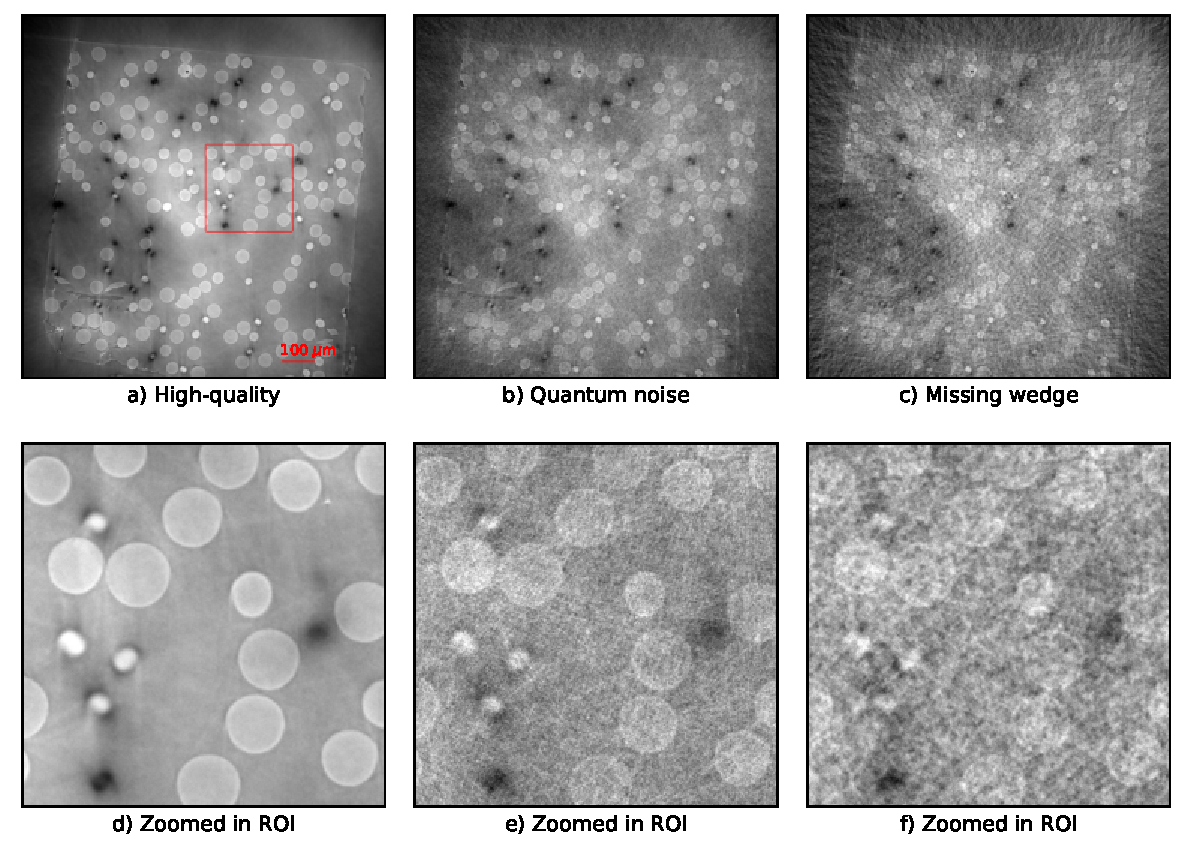
\includegraphics[width=.9\textwidth]{figures/noisecomparison.pdf}
    \caption[Reconstruction noise comparison]{Comparison of a high-quality reconstruction, a quantum noise reconstruction, and a missing wedge reconstruction. Images d), e), and f) are zoomed in \acrshort{roi}s of images a), b), and c) respectively. The \acrshort{roi} is marked in a). The quantum noise is simulated by applying Poisson noise to the sinogram before reconstruction, and the missing wedge problem is simulated by selecting a subsampling of every 32nd projection from the high-quality reconstruction. The images are of a central slice from the dataset tomo\_00058 \cite{datasetglassspheres} reconstructed using \acrshort{fbp} from TomoPy \cite{TomoBank}. }
    \label{fig:noisecomparison}
\end{figure}

\section{Imaging Method}
\todo[inline]{Keep this section?}
\subsection{Setup}
\missingfigure{Figure of generic CT setup, if section is staying. }

\section{Reconstruction}
After acquiring the attenuation coefficient projections, or sinograms, this data must be reconstructed into an image (of either 2D or 3D) of the object. The collection of a sinogram $P_\theta$ for projection angle $\theta$ is given by the Radon transform \cite{4307775,jimaging4110128}
\begin{equation}
    \label{eq:radontransform}
    P_\theta(u) = \iint f\left(x,y \right)\delta\left(x \cos \theta + y \sin \theta -u \right)dxdy,
\end{equation}
where $u$ is the position on the detector and $\delta$ is the Dirac delta function. In practice, because of computational and instrumental limitations, the projection data are acquired only for a limited number of projections $N_\theta$ as well as $N_d$ detector elements, and the imaged object is represented by a pixel grid of size $N \times N$. Thus, the acquired projection data is described by a vector $\bm{y} \in \mathbb{R}^{N_\theta \times N_d}$, the reconstructed image by a vector $\bm{x} \in \mathbb{R}^{N \times N}$, and the formation of the projection data can be stated as a linear system \cite{jimaging4110128}
\begin{equation}
    \label{eq:projectiondata}
    \bm{y} = \bm{A}\bm{x},
\end{equation}
where element $a_{ij} \in \mathbb{R}$ of $\bm{A} \in \mathbb{R}^{N_\theta N_d \times N^2}$ is equal to the contribution of image pixel $j$ to detector pixel $i$. This gives the tomographic reconstruction problem of recovering the unknown object $x$ from the acquired projection data $y$. It can be seen as performing the inverse Radon transform, which is known to be an ill-posed inverse problem \cite{KabanikhinIllVersed,GANrec}\footnote{Inverse problems are often ill-posed. An ill-posed problem is a problem that does not meet any one or more of the three conditions suggested by Jacques Hadamard: existence, uniqueness, and stability \cite{KabanikhinIllVersed}. The stability condition is most often violated. This means that its output is highly sensitive to small changes in the input (e.g. noise can drastically change the resulting output). }. 

Tomographic reconstruction algorithms are generally divided into two groups: direct reconstruction, and iterative reconstruction, however a third method using \acrshort{ml} has also shown some promise \cite{GANrec}.

\subsection{Direct Reconstruction}
Direct tomographic reconstruction algorithms are based on finding a continuous inversion formula of the continuous forward Radon transform, as given in \cref{eq:radontransform}, and discretizing the result \cite{jimaging4110128}. The most commonly used direct reconstruction algorithm is the \acrfull{fbp} algorithm, which can be written as \cite{jimaging4110128}
\begin{equation}
    \label{eq:fbp}
    \bm{x}_{FBP} = \bm{A}^T \bm{C}_h \bm{y},
\end{equation}
where $\bm{C}_h$ is a 1D convolution operation that convolves each detector row in $\bm{y}$ with a filter $\bm{h} \in \mathbb{R}^{N_d}$. The filter is typically some standard filter that can be used for any reconstruction (e.g. the Ram-Lak filter), and may include low-pass filtering to reduce high frequency noise in the reconstructed image \cite{681991}. It has also been shown that this filter can be learned by use of \acrshort{ml} (more specifically an \acrshort{ann}) to further improve the performance of \acrshort{fbp} \cite{6607157}. 

Direct algorithms, such as \acrshort{fbp}, have the advantage of most often being computationally efficient, as well as producing accurate results when enough projections are available \cite{jimaging4110128}. The issue with these techniques arises when a limited number of projections are available, as they are generally highly prone to noise leading to insufficient image quality for proper analysis \cite{jimaging4110128}. This is where the use for iterative reconstruction algorithms arises.

For \acrshort{ct} imaging systems where the X-ray beam is conical (as opposed to parallel), an alternative direct reconstruction method similar to \acrshort{fbp} is the \acrfull{fdk} reconstruction algorithm \cite{Feldkamp:84}. 

\subsection{Iterative Reconstruction}
Iterative tomographic reconstruction algorithms are based on iteratively solving the linear system given in \cref{eq:projectiondata}. A common method used is to try and find reconstructed images that minimize the $l^2$-norm of the residual error (i.e. the difference between the acquired sinograms, and the Radon transform of the reconstructed image\footnote{Calculating the inverse Radon transform is an ill-posed problem and is challenging, however calculating the Radon transform itself is an easy task. }) as well as an additional term $g$ that penalizes images that do not confine to some prior knowledge or assumption of the imaged object. This process can be written as \cite{jimaging4110128}
\begin{equation}
    \label{eq:iterativesolution}
    \bm{x}_{iter} = \underset{\bm{x}}{\text{argmin}} \left|\left|\bm{y} - \bm{A}\bm{x}\right|\right|_2^2 + \lambda g(\bm{x}),
\end{equation}
where $\left|\left| \bm{\cdot} \right|\right|_2^2$ denotes the $l^2$-norm, and $\lambda$ is the relative weight of the prior knowledge penalty compared to the residual error. If a prior knowledge penalty that fits a reconstruction well is chosen, iterative reconstruction algorithms can produce significantly more accurate reconstructions than direct methods when reconstructing from limited data \cite{jimaging4110128}. If the chosen prior knowledge penalty does not fit well however, or if the weighting parameter $\lambda$ is poorly selected as it is a problem-dependent parameter, it may lead to poor quality reconstructions. 

A large drawback with iterative reconstruction is its (often) large computatinal cost. These types of reconstructions are slower, which may make it difficult to apply them to time-sensitive real-world tomographic data \cite{jimaging4110128}. Newer and more powerful computers can to some extent offset this downside to iterative reconstructions \cite{willemink2013iterative}. 

Because of these limitations and drawbacks, direct reconstruction algorithms are still often preferred in many fields \cite{Pan_2009}. 

Another iterative reconstruction algorithm is known as \acrfull{piccs} \cite{piccs}. It is used to better reconstruct datasets that are limited in the number of projections available when multiple imagings have been done for several time frames (known as dynamic \acrshort{ct} imaging). By reconstructing a prior image from the union of interleaved datasets from several time frames, the \acrshort{piccs} reconstruction algorithm utilizes the spatial-temporal correlations in the imaging to make assumptions on the imaged object. The prior image is used as a constrain on the reconstruction of the missing wedge reconstructions. 


\subsection{Other Methods}
In addition to direct and iterative reconstruction techniques, \acrshort{ml} has been used to make an iterative-like reconstruction algorithm \cite{GANrec}. One method, termed GANrec, is based on a \acrshort{gan} (which will be introduced in \cref{sec:ml:types:gan}) and is an \acrshort{ml} method that does not require training of the network before reconstruction, instead using the training process as the reconstruction process. 

It takes a given sinogram $\bm{y}$ and uses the generating network $G$ to create a candidate reconstructed image $\bm{x} = G(\bm{y})$, then creates the corresponding candidate sinogram $\hat{\bm{y}} = P(\bm{x})$, where $P$ is the Radon transform. The loss $L = \left|\left| y - \hat{y} \right|\right|$ is then the basis of training the network (i.e. reconstructing the image)\footnote{The actual loss used for training GANrec also includes an adversarial loss, which will be introduced in \cref{sec:ml:training:lossfunctions}, however it is omited in this description for the sake of simplicity. }.

The sinogram-to-reconstruction transformation cannot be done by a conventional \acrshort{cnn}-style network, however it has been shown that a single fully connected layer can perform this transformation \cite{PASCHALIS2004211}. The accuracy of the transformation can be improved by increasing the number of layers and neurons, however this is dependent on the available computational power \cite{GANrec}. Because of this limitation, the generating network in GANrec is a modified version of U-net \cite{unet}, which will be introduced in \cref{sec:ml:types:encoderdecoder}, with three fully connected layers at the start to perform this transform. 
\chapter{Machine Learning}
\label{sec:ml}
The field of \gls{ml} is often seen as a part of the greater field of \gls{ai}\cite[3]{Alpaydin10}, and the term was coined by Arthur Samuel in \citeyear{samuelmachinelearning} \cite{samuelmachinelearning}. An \gls{ml} algorithm builds a model based on a dataset, intended to make predictions or classifications without being explicitly programmed how to do so. 

Whereas some problems can easily be solved by programming an explicit algorithm (e.g. sorting a list, or \gls{fbp} reconstruction), there are many cases where an exact algorithm fails to provide adequate solutions to the problem. A typical example is to filter out spam emails from an email inbox. The content and structure of the spam emails vary sufficiently to prevent filtering them with "hardcoded" rules, as in conventional algorithms. This is where \gls{ml} comes in: an \gls{ml} model can be trained to discern differences in a dataset without being explicitly told what to look for. So long as there is a sufficient amount of data to train the model with, it may be able to find a pattern in the data and thereby predict or classify new data, or augment or enhance the data \cite[2-4]{Alpaydin10}. 

There are many different \gls{ml} algorithms, however in this thesis, only the class of \textit{neural networks} will be discussed and the focus will be on \textit{supervised learning}. 

This chapter contains a brief introduction to neural networks and their basic components, an explanation of what a \acrlong{cnn} is, a description of encoder-decoder networks, and an introduction to \acrlong{gan}s, before covering the basics of how a neural network is trained and giving an overview of some common loss functions used for this process. 

\section{Components of a Neural Network}
\label{sec:ml:componentsofaneuralnetwork}
\todo[inline]{Briefly state what a neural network is. }
Neural networks were initially designed to simulate the human brain and how it learns and adapts to new information \cite{McCulloch1943}. Because of this, the basic building block of a neural network is called a neuron. Several neurons build up a layer, and several layers build up a neural network. Neurons in different layers have connections to each other (i.e. neurons in layer 1 are connected to neurons in layer 2), and these connections have weights and biases. A simple schematic of this can be seen in \cref{fig:neuralnetwork}. The value of a neuron is a real number and can be given as \cite[81]{Wang2003}
\begin{equation}
    \label{eq:neuron}
    Y_{k} = \sigma\left(\sum_{j=0}^{m}w_{kj}x_j + \lambda \right),
\end{equation}
where $k$ refers to which neuron it is, $m$ is the number of inputs to the neuron, $w_{kj}$ is the weight of connection $j$, $x_j$ is the output value of neuron $j$ into neuron $k$, $\lambda$ is a bias term, and $\sigma$ is the activation (or transfer) function, which will be introduced later. It is thus a weighted sum of the values of the neurons in the previous layer (or more precisely, of all the input neurons to a given neuron, which often is the previous layer). Note that this describes a simple fully connected feedforward \gls{ann}, more precisely a multilayer perceptron, and other types of neural networks may contain other types of layers \cite{oshea2015introduction}. 

\begin{figure}[htbp]  
    \centering
    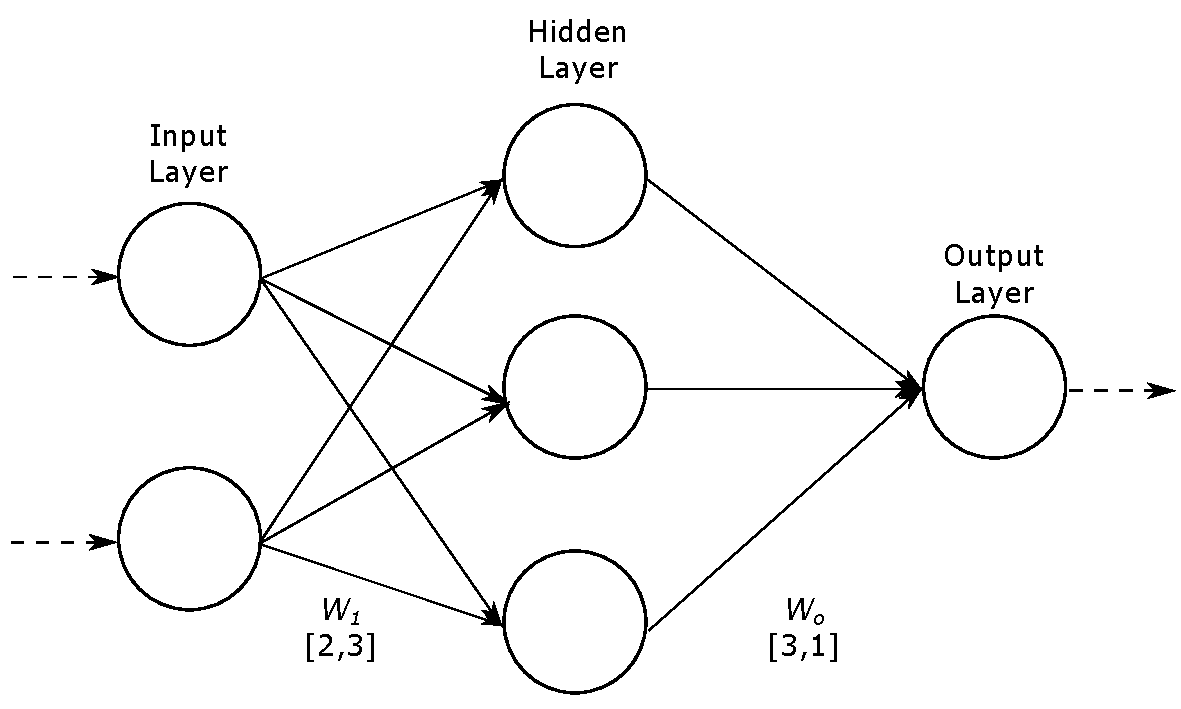
\includegraphics[width=.8\textwidth]{figures/neuralnetwork.pdf}
    \caption[Neural network example]{A simple schematic of a neural network. Each circle represents a neuron, the solid arrows represent connections between neurons, and the dotted arrows represent input and output channels. The dimensions of the network parameters are denoted as $W_n$, where $n$ refers to the layer the parameters input into. This network specifically is a fully connected feedforward \acrlong{ann} with one hidden layer. }
    \label{fig:neuralnetwork}
\end{figure}

The activation function, also known as the transfer function, is denoted as $\sigma$. Its purpose is to bound the value of a neuron so that the network is not crippled by divergent neurons \cite[81]{Wang2003}. There are many different activation functions, and some examples are presented in \cref{tab:activationfunctions} and plotted in \cref{fig:activationfunctions}. Furthermore, the activation function is used to introduce nonlinearity to the network,\footnote{For this reason, the identity activation function $f(x)=x$ generally performs poorly.} and it can be shown that a two-layer deep neural network with a nonlinear activation function is a universal function approximator \cite{Cybenko1989}. 

\begin{table}[htbp]
    \centering
    \caption[Activation functions]{Overview of some of the commonly used activation functions in neural networks. }
    \label{tab:activationfunctions}
    \begin{tabular}{ll}
    \hline
    Name & Function, $f(x)$ \\
    \hhline{==}
    Identity & $x$ \\
    Rectified Linear Unit (ReLU) & $\max\left(0, x\right)$ \\
    Leaky Rectified Linear Unit (LReLU) & $\max\left(\alpha x, x\right), \alpha\in[0,1]$ \\
    Logistic/soft step & $\frac{1}{1+e^{-x}}$  \\
    tanh & $\frac{e^x - e^{-x}}{e^x + e^{-x}}$ \\
    Softplus & $\ln\left(1+e^x\right)$ \\
    \hline
    \end{tabular}
\end{table}

\begin{figure}[htbp]  
    \centering
    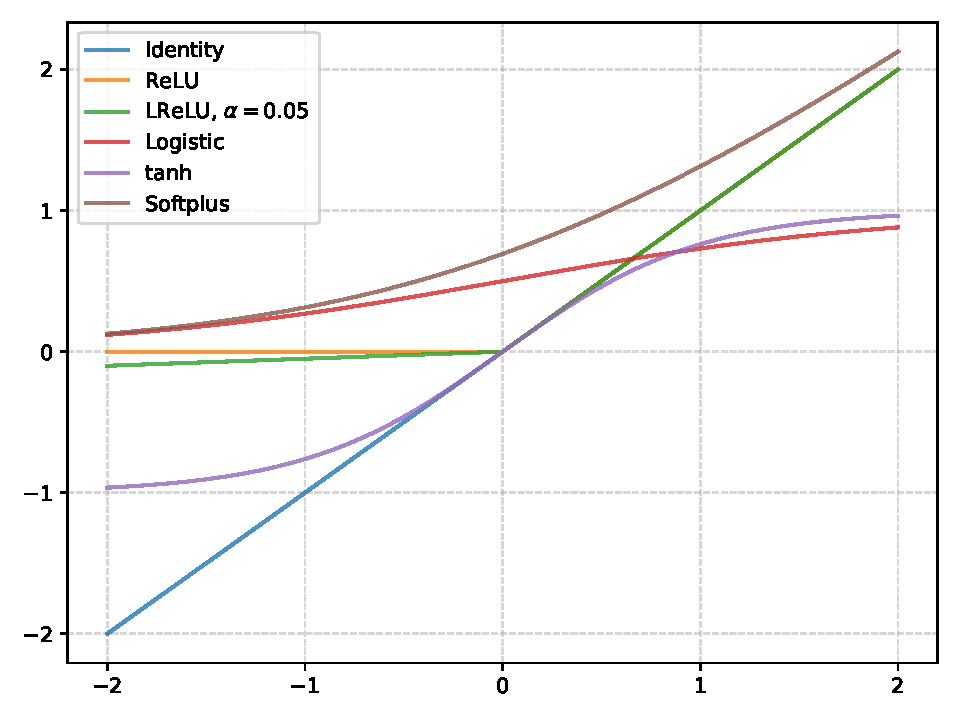
\includegraphics[width=.8\textwidth]{figures/activationfunctions.pdf}
    \caption[Activation functions]{Plot showing a selection of activation functions for $x\in[-2,2]$. Note that identity, ReLU, and LReLU are overlapping for $x\in[0,-2]$. }
    \label{fig:activationfunctions}
\end{figure}

The output of a neural network can be defined to be any shape (e.g. a vector, or matrix). In \cref{fig:neuralnetwork} the output is a single value, however it could just as well have been defined as a vector. If the output is a single value it can for instance be interpreted as a probability, however if it is a vector of length $n$ it can be seen as $n$ probabilites of different events or features. The output of a neural network is often called a feature map, because it can be seen as a mapping of the features of the input data. 

For example, if a neural network is trained with a dataset containing images of handwritten digits $0-9$, an output with a size of $10$ could contain probabilities of a given image containing a specific digit where each output value is the probability of one digit. One well-known dataset that is often used for this exact problem is the MNIST dataset \cite{mnist}.


\section{Neural Network Types}
There are many different types of neural networks that are suited for different problems. Here, a selection of types that lead up to the \gls{gan} structure used in this thesis will be introduced. 

\subsection{Convolutional Neural Network}
A \gls{cnn} builds upon the structure of the \gls{ann}, however it adds a new type of layer: the convolutional layer. Instead of containing a set of neurons, this layer contains one (or more) convolutional kernel(s), and performs a convolution of the input to the layer with the kernel(s). This type of network was first introduced in \citeyear{lecun1999object},\footnote{There is some disagreement around whether the paper by LeCun in \citeyear{lecun1999object} \cite{lecun1999object} was truly the introduction of \gls{cnn}s, however it is often seen as it. } and has shown to perform well for many different image related tasks \cite{lecun1999object,alexnet}. The convolution operation allows the network to utilize 2D information by performing 2D convolutions.\footnote{Likewise higher-dimensional information may be used by performing higher-dimensional convolutions \cite{8353466}. } This has been shown to perform exceptionally well in image processing tasks \cite{alexnet,oshea2015introduction}\todo[]{"Examples with refs." meaning what? Should I mark these refs. as examples? If so, how?}.

The discrete convolution operator is defined as \todo[]{Reference}
\begin{equation}
    \label{eq:convolution}
    g(x,y) = \omega \ast f(x,y) = \sum_{dx=-a}^{a}\sum_{dy=-b}^{b} \omega(dx,dy)f(x+dx,y+dy),
\end{equation}
where $g(x,y)$ is the convoluted matrix, $f(x,y)$ is the original matrix, and $\omega$ is a convolution kernel of dimension $(2a+1,2b+1)$.\footnote{The dimensions of the kernel are typically square and odd, such as $3\times3$ or $5\times5$, giving $dx,dy\in[-1,1]$ or $dx,dy\in[-2,2]$. } For the sake of simplicity, kernel dimensions will be referred to as $a\times b$ where $a$ and $b$ simply represent the kernel dimensions, and not the half-dimension as would correspond to \cref{eq:convolution}. 

A visualization of the convolution of a matrix (which could represent an image) with a given kernel is provided in \cref{fig:convolution}. Here, the kernel dimensions are $3\times3$. The output matrix has reduced dimensions corresponding to the kernel dimensions. The reduction can be given as 
\begin{equation}
    \left( x_o,y_o \right) = \left( x_i - \left(a - 1\right), x_i - \left( b - 1 \right) \right),
\end{equation}
where $(x_o,y_o)$ are the output dimensions, $(x_i,y_i)$ are the input dimensions, and $a$ and $b$ are the kernel dimensions. In some situations it may not be wanted to reduce the dimensions of the input, and padding the input with zeroes on all sides can be used to combat this. This technique is called zero-padding \cite{oshea2015introduction}. 
\begin{figure}[htbp]  
    \centering
    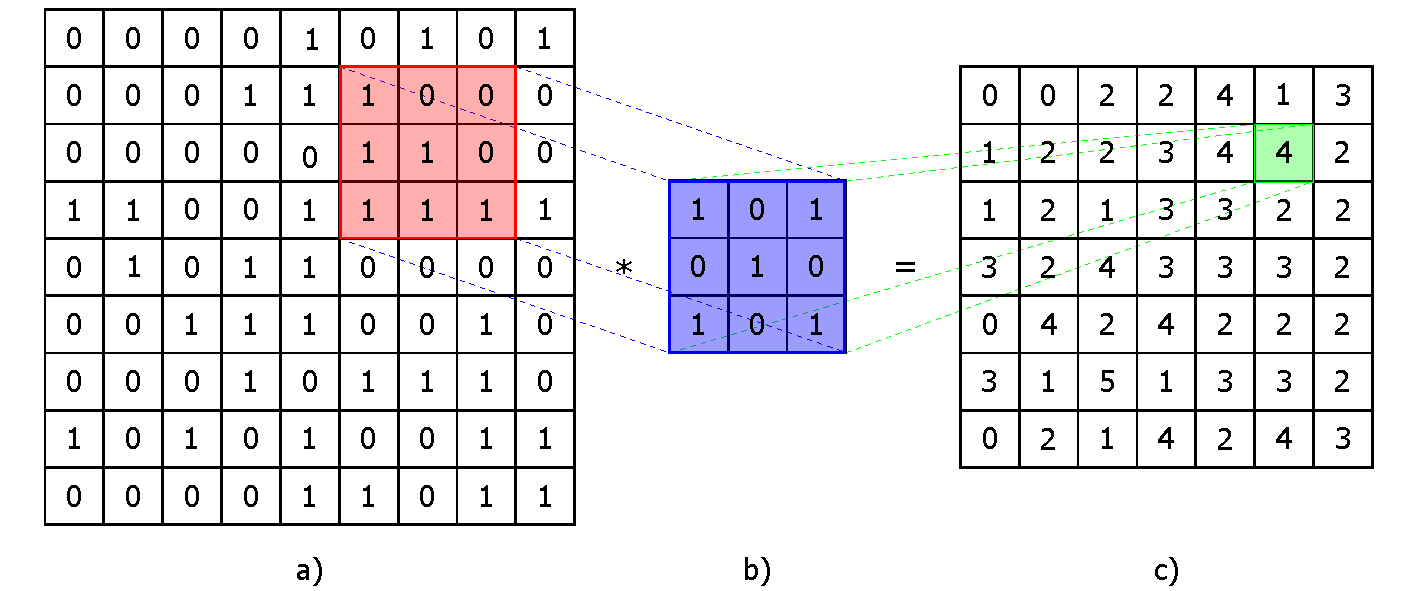
\includegraphics[width=.85\textwidth]{figures/convolution.pdf}
    \caption[Convolution example]{An example showing how a convolution works. This figure depicts: a) an input matrix of dimension $(9,9)$ (e.g. an image), b) a $3\times3$ convolutional kernel, and c) the resulting convolution of dimension $(7,7)$. This convolution also has a stride of 1. Note that the output dimension is smaller than the input dimension. }
    \label{fig:convolution}
\end{figure}

Multiple convolutional kernels can be used in parallel in each convolutional layer. The number of kernels is then referred to as the number of channels. 

The stride of a convolution is how far the kernel shifts \cite{oshea2015introduction}. In the example given in \cref{fig:convolution}, the stride is 1. If the stride were set to 2, the kernel would shift two units in the matrix for each output. This would mean less overlap between each value in the output, but also further reduction of the output dimensions. 

Often, pooling layers are included in \gls{cnn}s. These layers are used to down sample the feature maps after a convolutional layer by applying some pooling function (e.g. max, average, sum) to an area of the feature map, reducing the dimension. This can for instance be a $2\times2$ max pooling layer that looks at a $2\times2$ section of a feature map and replaces it with a single value corresponding to the maximum value of the original section. Pooling layers reduce the dimensions of the feature map corresponding to the size of the pooling (e.g. a $2\times2$ pooling layer reduces both dimensions of a feature map by a factor of $2$). 

The part of the convolution that a \gls{cnn} learns is the values in the convolutional kernel. Each layer of the \gls{cnn} may have several kernels that are applied in parallel (e.g. 32 kernels applied to the same input). Each kernel is often called a filter. One of the advantages of using convolution in neural networks is the reduction in the number of trainable parameters: a typical convolutional kernel contains $9-49$ parameters (for kernels of dimensions $3\times3$ to $7\times7$), however a fully connected feedforward network may have several thousand parameters for each layer.\footnote{Consider an image of dimension $100\times100$. In a fully connected \gls{ann} there would have to be $100 \cdot 100 = 10^4$ connections from each neuron in one layer to the next layer for a total of $10^{8}$ connections, where each connection has a trainable parameter. In comparison, if using a \gls{cnn} with 32 channels (or kernels) of dimension $3\times3$ there are only a total of $32 \cdot 3 \cdot 3 = 288$ trainable parameters. } 
\todo[inline]{Write about overfitting? Reduce number of trainable parameters helps avoid overfitting. }

\subsection{Encoder-Decoder Network}
\label{sec:ml:types:encoderdecoder}
An encoder-decoder network is a type of \gls{ann} that learns to copy its input to its output \cite{https://doi.org/10.1002/aic.690370209}. It consists of two parts (as the name suggests): an encoder, and a decoder. The task of the encoder is to take the input and encode it into a feature map. The decoder then takes the resulting feature map and decodes it into an output similar to the original input. A schematic of this structure can be seen in \cref{fig:encoderdecoder}. The encoder's goal is to extract the relevant information from the input, ignoring any signal noise or unwanted data. The decoder then recreates something similar to the original data from the "denoised" feature map. It is common to use \gls{cnn}s as both encoder and decoder, where consecutive layers in the encoder reduce the dimensions of the feature maps and consecutive layers in the decoder increase the dimensions of the feature maps. Encoder-decoder networks have been shown to perform well in many different tasks, such as image segmentation \cite{7803544} and PET image reconstruction \cite{HAGGSTROM2019253}.  

\begin{figure}[htbp]  
    \centering
    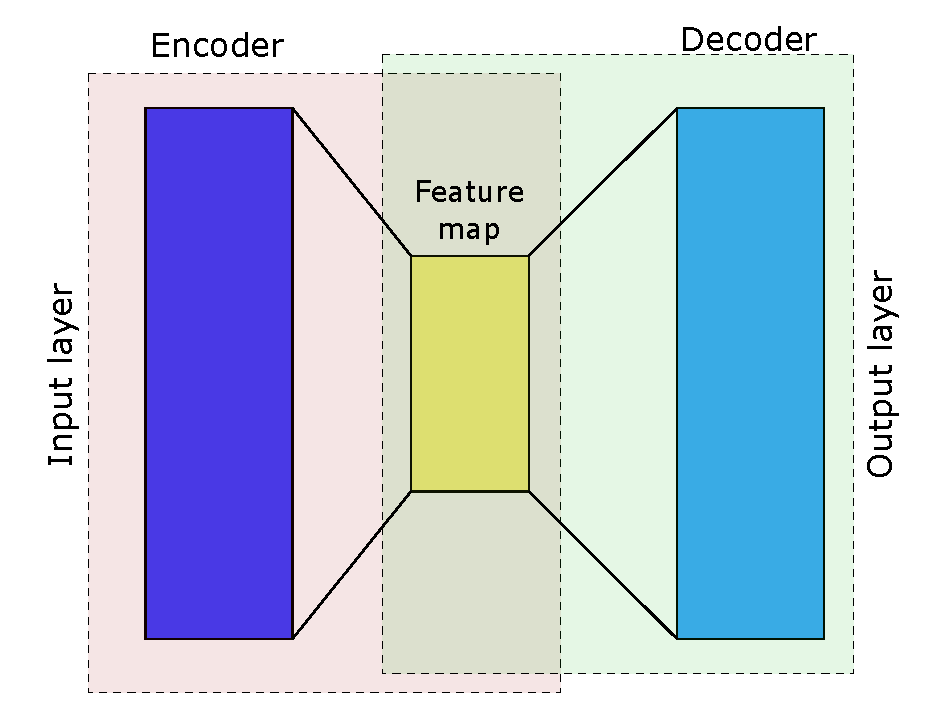
\includegraphics[width=.7\textwidth]{figures/encoderdecoder.pdf}
    \caption[Encoder-decoder network]{A simple schematic of the overall structure of an encoder-decoder network. It consists of two separable networks, the encoder and the decoder, working together. The input and output layers are of the same dimensions. }
    \label{fig:encoderdecoder}
\end{figure}

In an encoder-decoder network, the encoder and decoder are two separate networks that can work independently of each other. Another similar network structure that builds upon the encoder-decoder is the U-net convolutional network, originally proposed for biomedical image segmentation \cite{unet}. It also contains an encoder and a decoder part, however the two networks are not separable as there are skip-connections between layers in the encoder and layers in the decoder. In a normal encoder-decoder network there is first one mapping from the input $X$ to the feature map $L$, $X \mapsto L$, and then a mapping from the feature map $L$ to the output $Y$, $L \mapsto Y$. These two mappings are not dependent on each other. In the U-net architecture however,  the mapping in the decoder also depends on the input $X$, making it $[X+L] \mapsto Y$. 


\subsection{Generative Adversarial Network}
\label{sec:ml:types:gan}
\gls{gan}s were introduced in \citeyear{goodfellow2014gan} by Goodfellow et al.  as a novel method of estimating generating models via an adversarial process \cite{goodfellow2014gan}. This type of neural network consists of two separate networks: a generator and a discriminator. The generator, called $G$, captures the distribution of the training data and generates new samples from that distribution, while the discriminator $D$ estimates the probability that a given sample came from the training data (i.e. is a real sample) rather than being a generated sample from $G$. 

The two networks play a game where they try to minimize their own cost, or error rates, while at the same time maximizing the other network's cost \cite{goodfellow2020gan}.\footnote{\gls{gan}s are designed to reach a Nash equilibrium at which neither of the two networks can reduce its costs without changing the other network's parameters \cite{liu2020tomogan}.} As opposed to normal neural networks that are based on optimization to reduce their error rates, \gls{gan}s are based on game theory \cite{goodfellow2020gan}. 

To generate random samples from the distribution of the training data, a fully trained \gls{gan} is given random noise as input and then maps that to a random sample, such as in \cite{zhangsagan}. This allows the network to generate new samples that are similar, but not equal, to the training data. Another common use case for \gls{gan}s is to instead of feeding the network random noise as input, feeding it some data that needs augmentation. This has been used to denoise images and has been shown to be a viable method for image super-resolution \cite{8710893,Ledig_2017_CVPR}. 

\gls{gan}s are generally seen as unsupervised learning algorithms with a supervised loss as part of the training. For a general \gls{gan} the training data is an unlabeled dataset and the \gls{gan} tries to model a probability distribution of the dataset in order to randomly generate new samples. By generating new samples, it is trivial to apply labels to the original (i.e. real) an generated samples and then use these labels to perform supervised learning to train the discriminator. 

When the input dataset to the \gls{gan} no longer only contains a set to learn the distribution of, but instead the \gls{gan} training process is used to train a generator that takes a non-random input and outputs an augmented version of the input (such as in \cite{liu2020tomogan}), it can be seen as a supervised learning algorithm.

\section{Training a Neural Network}
The process of tuning all the parameters (i.e. weights and biases) of a neural network is called training. During training, input data from a training dataset is forwards propagated through the network, and the resulting feature map is compared to an expected feature map (e.g. manually labeled data).\footnote{This is what is called supervised learning, as opposed to unsupervised learning where there is no ground truth answer to compare to, instead trying to learn some inherent structure of the data without explicit labels (e.g. clustering). } The difference in these feature maps is calcuated using some loss function, and the loss is then backward propagated through the network to update each and every parameter to reduce the loss. 

Generally, the entire training dataset is repeatedly passed through the network multiple times. Each full runthrough of the training dataset is called an epoch of training. This however can often introduce a problem: the training dataset can typically not fully fit in the computer memory at once. Therefore it is divided into mini batches, and after each mini batch the weights are adjusted. The propagation of one mini batch is often called one iteration, and thus one epoch consists of several iterations. The size of a mini batch is a tunable parameter, however typically it is in the range of $32-512$ (e.g. 128 in the well-known article by A. Krizhevsky et al. \cite{alexnet}).\footnote{There is ongoing research into techniques to increase the batch size by several orders of magnitude as larger batches allow for easier parallelization, however large batch sizes have been shown to cause instability during training \cite{you2017large}. } The size of a mini batch can sometimes also be referred to as the batch size. 

\subsection{Hyperparameters}
During training, the parameters of the neural network are automatically changed, however there are some parameters that are set manually beforehand. These are called hyperparameters \cite{claesen2015hyperparameter}. Some typical hyperparameters are:
\begin{itemize}
    \item Number of layers (i.e. depth of network).
    \item Size (or dimensions) of layers.
    \item Learning rate.
    \item Number of iterations to train the network (i.e. number of epochs).
    \item Mini batch size.
\end{itemize}

The process of choosing these hyperparameters is not an exact science, and there is research being done into finding ways of automatically tuning hyperparameters to their ideal configurations, called hyperparameter optimization \cite{hyperparameteroptimizing}.

\subsection{Loss Functions}
\label{sec:ml:training:lossfunctions}
To properly quantify the error, or loss, of a neural network one needs to define some metric. These are called loss functions. Depending on the problem type diferent loss functions may perform better than others, however there are some standard loss functions often used. Some of these, as well as some specific ones used in this thesis, will be presented here. The losses are calculated on a per-pixel basis and summed unless otherwise stated. 

Perhaps the most commonly used loss function is the \gls{mse}. It is closely related to the L2-norm,\footnote{Sometimes the \gls{mse} loss is improperly called the L2-norm, however that is incorrect. The L2-norm can be defined as the square root of \gls{mse}. } and it can be defined as
\begin{equation}
    \label{eq:lossmse}
    L_{\text{MSE}} = \frac{1}{N} \sum_{i=1}^N(Y_i - \hat{Y}_i)^2,
\end{equation}
where $Y$ is the correct (labeled) value,  $\hat{Y}$ is the predicted value, and $N$ is the number of samples. This often performs well, however in cases such as image processing or image super-resolution it has shown to cause blurring \cite{7797130}.

Another similar loss function is the \gls{mae}, which is closely related to the L1-norm. It can be defined as
\begin{equation}
    \label{eq:lossmae}
    L_{\text{MAE}} = \frac{1}{N} \sum_{i=1}^N |Y_i - \hat{Y}_i|,
\end{equation}
with $Y$ and $\hat{Y}_i$ being the same as previously defined. This loss function does not over-penalize larger errors, and therefore may have different convergence properties than \gls{mse} \cite{7797130}. It has been shown to perform better than \gls{mse} in some image processing cases \cite{7797130,10.1002/mp.13713}. 

\todo[inline]{Write something about general norms for loss functions? }
% These loss functions can be generalized from $L1$ and $L2$ norms to $Ln$ norms

A more recently introduced loss function is the log-cosh loss function, defined as \cite{chen2019log}
\begin{equation}
    \label{eq:losslogcosh}
    L_{\text{Log-cosh}} = \frac{1}{a} \sum_{i=1}^N \log ( \cosh ( a ( Y_i - \hat{Y}_i))),
\end{equation}
where $Y$ and $\hat{Y}$ are as previously defined, $\log$ is the logarithm, $\cosh$ is the hyperbolic cosine function, and $a$ is some positive hyperparameter $a \in \mathbb{R}^+$. It behaves similar to \gls{mse} around the origin, and similar to \gls{mae} at other points. It has been shown to perform well in image processing-related tasks \cite{7797130}.
% MSE, MAE, LogCosh, VGG, Adversarial
\todo[inline]{Wasserstein distance (for WGAN?)}
All the aforementioned loss functions rely on pixel-wise losses. Another type of loss function that has shown to perform well in image processing-related tasks is the use of a \textit{feature space-based loss} \cite{vggloss}. In the case of image processing, it means that the loss is based on measuring the difference in the feature space of the inference of a pre-trained network. Here, the pre-trained VGG network is used to measure a visual loss \cite{simonyan2015deep}. This specific loss function is termed visual loss, or VGG loss, and is defined as \cite{vggloss,liu2020tomogan}
\begin{equation}
    \label{eq:lossvgg}
    L_{\text{VGG}} = \sum_{i=1}^{N} \sum_{j=1}^{W_f} \sum_{k=1}^{H_f} \left(V_{\theta_{\text{VGG}}} (Y_i)_{j,k} - V_{\theta_{\text{VGG}}} (\hat{Y}_i)_{j,k} \right)^2,
\end{equation}
where $Y$ and $\hat{Y}$ are as previously defined, $V_{\theta_{\text{VGG}}}(Y)$ is the VGG feature map representation of image $Y$, and $W_f$ and $H_f$ are the dimensions of the feature maps extracted by the pre-trained VGG network. The VGG network is trained with natural images, specifically the ImageNet dataset \cite{deng2009imagenet}, however it has been shown to work well as a feature extractor for \gls{ct} images \cite{8340157}. 

Specific to \gls{gan}s is the adversarial loss. It is a measure of how well the generator network is able to produce samples that the discriminator network is unable to distinguish from real samples. It can be written as \cite{liu2020tomogan}
\begin{equation}
    \label{eq:lossadv}
    L_{\text{Adv}} = -\frac{1}{N} \sum_{i=1}^{N} D\left(  \hat{Y}_i \right),
\end{equation}
where $\hat{Y}_i$ is the generated guess from the generator network, and $D$ is the discriminator network giving a binary classification $D\left(\hat{Y}_i \right) \in [0,1]$ depending on whether it believes the given image is a real or generated one. Minimizing this loss ensures that the generator network produces samples that have a similar feature map (when extracted by the discriminator network) to real samples, and this process is the basis of \gls{gan}s. 


\subsubsection{Weighted loss}
In practice it is common to use a weighted sum of different loss functions. 
An example containing \gls{mse}, log-cosh, and VGG loss can be given as
\begin{equation}
    \label{eq:weightedloss}
    L_{\text{Total}} = \lambda_{\text{MSE}}L_{\text{MSE}} + \lambda_{\text{Log-cosh}}L_{\text{Log-cosh}} + \lambda_{\text{VGG}}L_{\text{VGG}},
\end{equation}
where $\lambda_N$ is a hyperparameter controlling the weight of $L_N$. 

\subsection{Backpropagation}
Backpropagation is the name given to the process of calculating the needed updates to the parameters of a neural network to reduce the error rate, or loss, of the network. It consists of calculating the partial derivatives of the loss function for each parameter of the network, and then updating them accordingly \cite{Rumelhart1986}. 

The process of passing an input through a network to get some result (i.e. inference) can be seen as forwards propagating through the network. When updating the parameters of the network, a backpropagation algorithm begins by calculating the error of the neurons in the final layer of the network, and then working its way backward layer by layer. For each parameter, its contribution to the total loss of the network is calculated, and the gradient of this contribution is calculated. The backpropagation scheme itself does not update the parameters, but rather it finds what part of the loss corresponds to what parameter. An optimizer is then applied to update the parameters.

\subsection{Optimizers}
To calculate the updates to all parameters, some optimizing method must be used. Two of the most common ones will be briefly introduced here.

\subsubsection{Stochastic Gradient Descent}
The simplest type of optimizer that is often used in training neural networks is the \gls{sgd}. It is an iterative method for optimizing an objective function that has suitable smoothness properties (e.g. differentiability) \cite{stochasticgradientdescent}. It looks at the error in the feature map of the training network (when compared to the labeled ground truth), and calculates an approximation of the gradient needed to update all the weights in the network to reduce the error. Because of the use of mini batches during training of neural networks, the \gls{sgd} method only looks at a randomly selected subset of the whole training data and it is therefore called a stochastic method. The learning rate of \gls{sgd} is the step size used when updating the weights based on the calculated gradient.

\subsubsection{ADAM}
A more sophisticated optimization algorithm was introduced in \citeyear{kingma2015adam}, and is called ADAM. It is an algorithm for first-order gradient-based optimization of stochastic objective functions, based on adaptive estimates of lower-order moments \cite{kingma2015adam}. It can be seen as an extension to \gls{sgd}. While \gls{sgd} has one single learning rate, ADAM has one learning rate for each different parameter based on estimates of first and second moments of the gradients. 
\chapter{Method and Datasets}
\label{sec:method}
In this chapter, the specific neural network used to denoise \acrshort{ct} images will be introduced, some image comparison metrics will be given alongside a brief discussion of them, the used datasets will be described, and the method used to compile a given dataset into a suitable format for the neural network will be explained. 


\section{TomoGAN}
\label{sec:method:tomogan}
The denoising neural network used in this thesis is called TomoGAN \cite{liu2020tomogan}. It is a \acrshort{gan} where the generator is based on the U-net model \cite{unet}, and the input to the \acrshort{gan} is not some random noise but rather some noisy image. There are some key differences in the generator from the U-net model, namely \cite{liu2020tomogan}:
\begin{itemize}
    \item There are three (instead of four) down- and up sampling layers.
    \item All convolutions have zero-padding to keep image dimensions unchanged during convolutions.
    \item The generator input is a stack of $d$ adjacent slices where eight $1\times1$ convolutions are applied. 
\end{itemize}
In the down sampling part of the generator, three sets of two $3\times3$ convolutional layers with ReLU activation functions extract feature maps. Between each set of convolutional layers there is a $2\times2$ max pooling layer, for a total down sampling of $8$ leading to a feature map of size $1/8$ of the original image in either dimension (e.g. images of dimensions $1024\times1024$ will result in a feature map of dimensions $128\times128$). The number of channels in a convolutional layer changes throughout the network begining with $8$ channels, and the feature map after the down sampling process has $128$ channels. 

The up sampling part of the generator is symmetric to the down sampling part, containing three sets of two $3\times3$ convolutional layers. The max pooling layers are replaced by bi-linear interpolation layers that instead of reducing the size of the feature map, increase it. Again, all the convolutional kernels have kernels of size $3\times3$ and use ReLU activation functions. At each of the three sets of convolutional layers, the feature maps from the corresponding set in the down sampling section are concatenated to the feature maps outputted from the previous set of convolutional layers\footnote{These skip-connection, as they are often called, are what make this structure a U-net style network and not simply an encoder-decoder network \cite{unet}. }. Finally, a $1\times1$ convolutional layer with a ReLU activation function followed by a $1\times1$ convolutional layer with a linear activation function is used to combine all the channels into a final output image. 

Because of the three $2\times2$ max pooling layers the dimensions of the input images must all be divisible by $2^3=8$. 

A schematic of the generator of TomoGAN can be seen in \cref{fig:tomoganstructure}.

\begin{figure}[htbp]
    \centering
    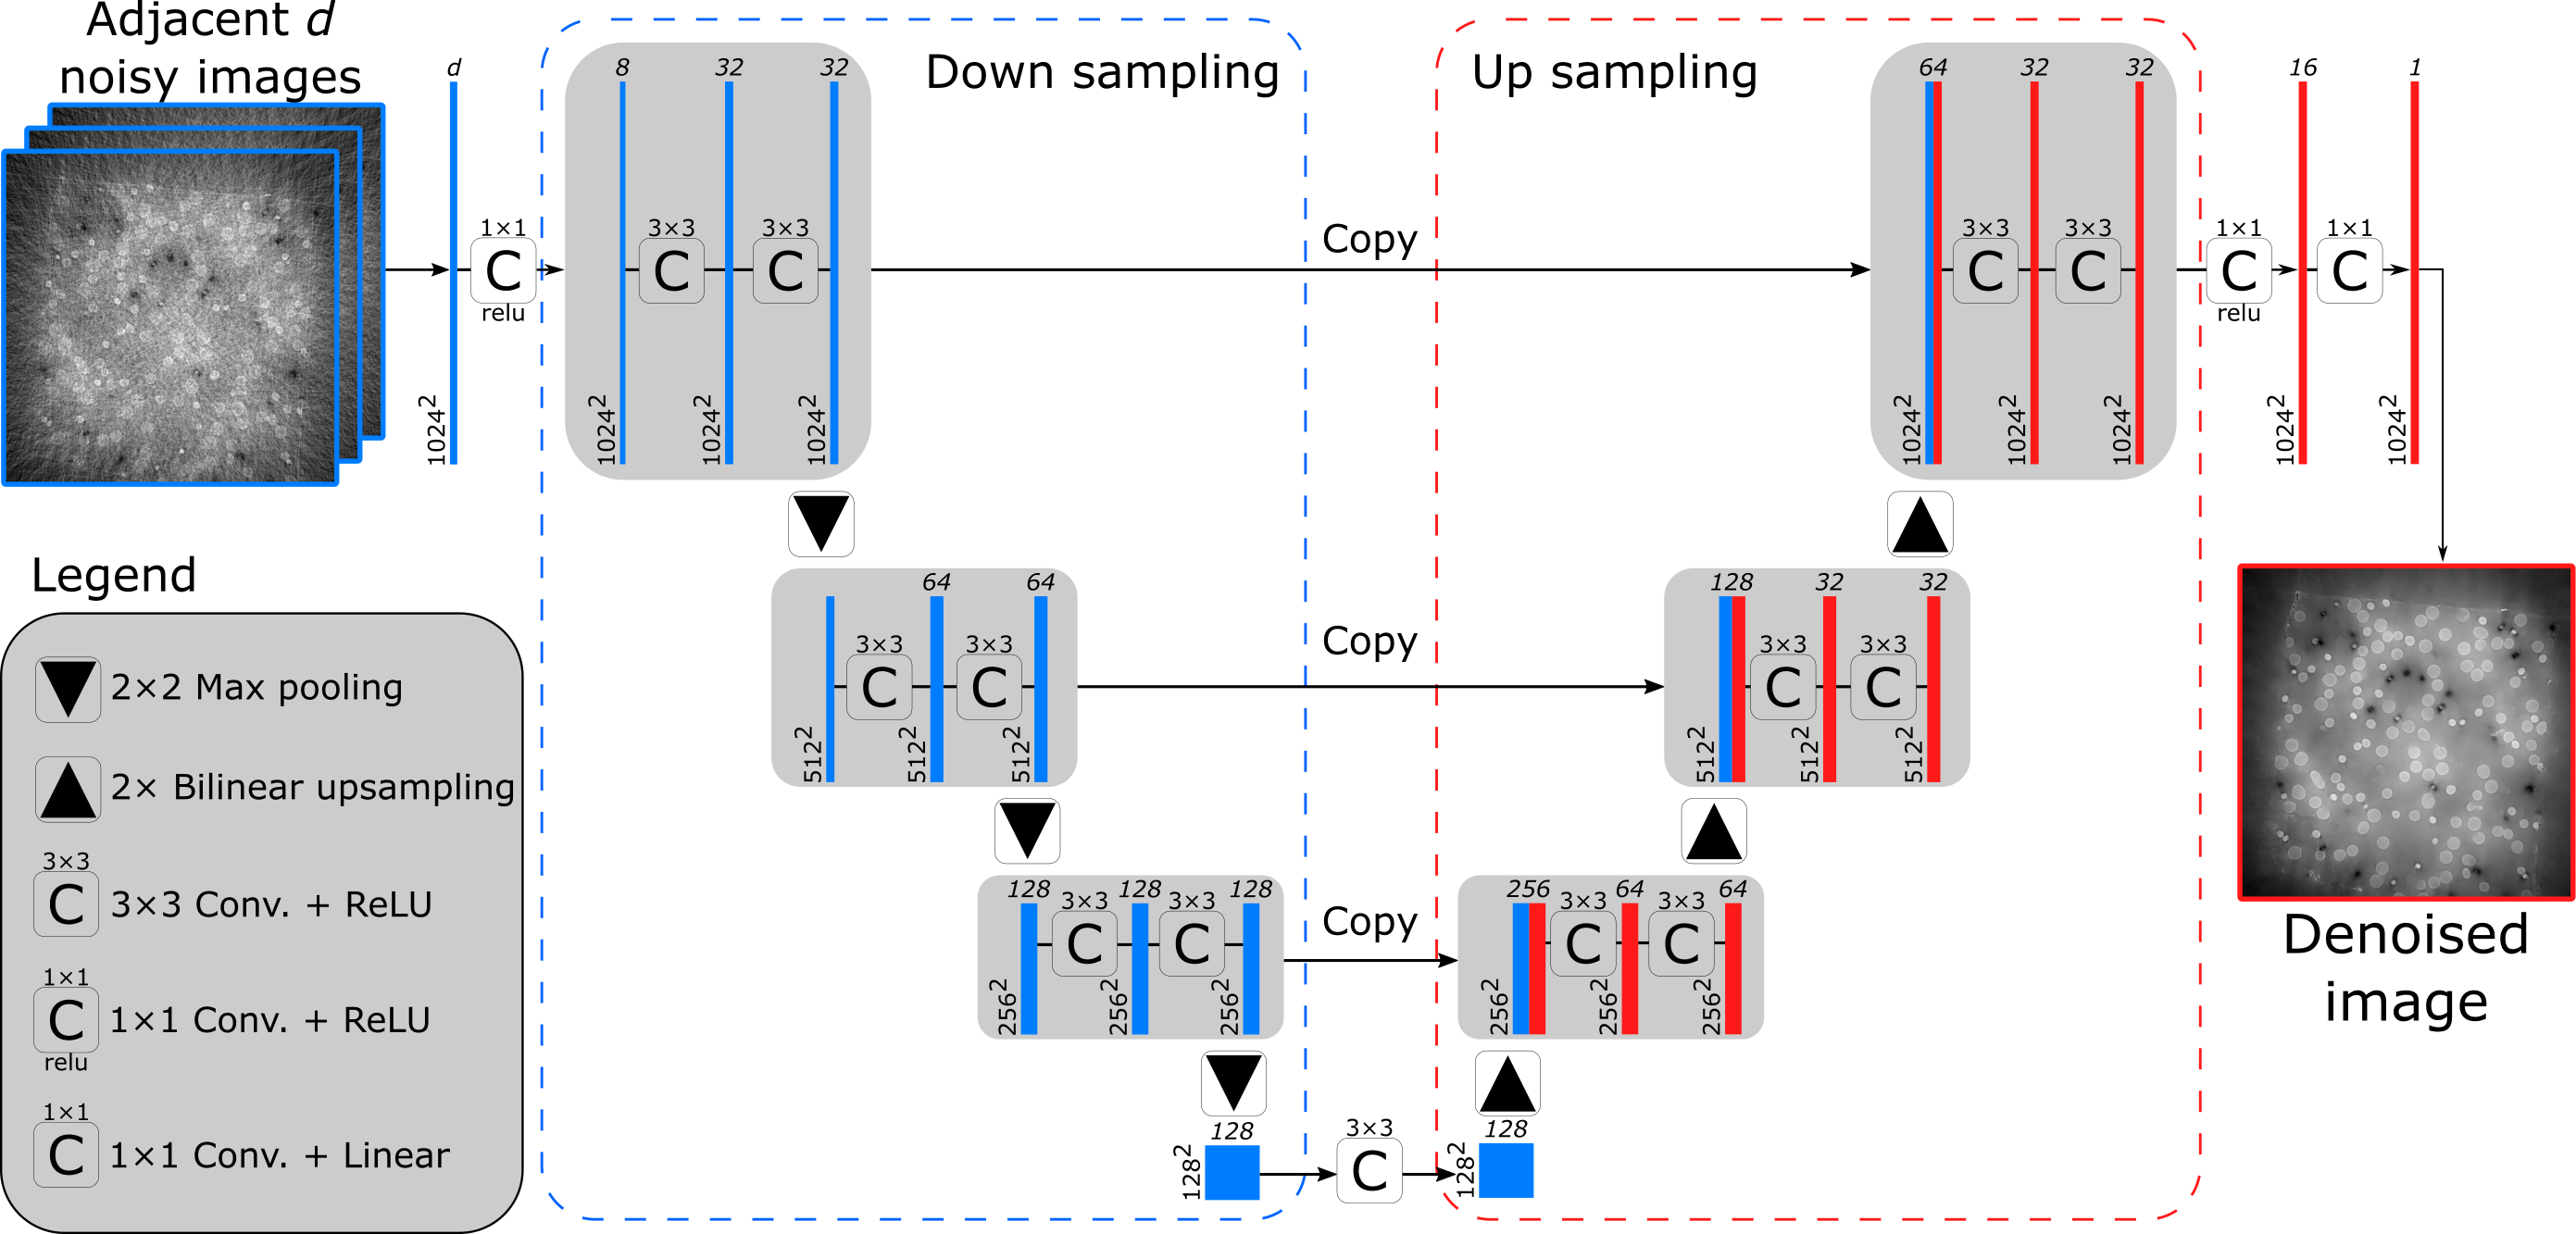
\includegraphics[width=0.95\textwidth]{figures/tomoganstructure.png}
    \caption[Visualization of the structure of TomoGAN]{A visualization of the structure of TomoGAN. Here, an image of size $1024\times1024$ has been used as an example. Every bar corresponds to a multi-channel feature map with the number of channels written above and the dimension of the feature map written on the bottom left. All convolutions use zero-padding. The type of activation function used with a given convolution can be seen in the legend. The copy operations transfer the feature map from a down sampling layer and concatenates it to the corresponding up sampling layer. } 
    \label{fig:tomoganstructure}
  \end{figure}

The discriminator network used to help train TomoGAN consists of six 2D $3\times3$ convolutional layers with leaky ReLU activation functions, as well as two fully connected layers. \todo[]{Write about Wasserstein distance and its use as loss function? }

No changes have been made to the structure of the TomoGAN network in this thesis, however some changes have been made to the loss function used to train the network. The original TomoGAN network, as given in \cite{liu2020tomogan}, was trained using a loss function comprising of an \acrshort{mse} loss, a feature based (VGG) loss, and an adversarial loss, given as 
\begin{equation}
    L_{\text{Total}} = \lambda_{\text{MSE}}L_{\text{MSE}} + \lambda_{\text{VGG}}L_{\text{VGG}} + \lambda_{\text{Adv}}L_{\text{Adv}}.
\end{equation}
Based on articles citing the log-cosh loss function as a good candidate for image processing \cite{7797130,chen2019log} it was added as an additional term to the total loss, giving the overall loss function
\begin{equation}
    L_{\text{Total}} = \lambda_{\text{MSE}}L_{\text{MSE}} + \lambda_{\text{Log-cosh}}L_{\text{Log-cosh}} + \lambda_{\text{VGG}}L_{\text{VGG}} + \lambda_{\text{Adv}}L_{\text{Adv}}.
\end{equation}
The weights for the different loss functions were mostly unchanged, with only $\lambda_\text{MSE}$ being slightly reduced to account for the fact that $L_\text{Log-cosh}$ covers a similar role (as they have similar activations). 

\section{Image Comparison Metrics}
\label{sec:method:metrics}
To properly quantify the performance of the denoising method, some metrics must be defined. While there are some standards to doing this, not all methods perform equally well. 

\subsection{Mean Squared Error}
\label{sec:method:metrics:mse}
The most commonly used full-reference image quality metric is the \acrfull{mse}, as defined (as a loss function) in \cref{eq:lossmse}. While it provides some sense of similarity and is very easy to calculate and physically understand, a low (i.e. good) \acrshort{mse} does not necessarily correspond to a high degree of visual similarity and it is therefore not a good metric to compare visual similarities in images \cite{413502,477498}. Likewise, the \acrfull{psnr}, which is another very commonly used metric, does not correspond to visual similarity. The \acrshort{psnr} can be defined from the \acrshort{mse}, and is given as \cite{477498}
\begin{equation}
    \label{eq:psnr}
    \text{PSNR} = 10 \cdot \log_{10} \left( \frac{\text{MAX}_Y}{MSE^2} \right),
\end{equation}
where $\text{MAX}_Y$ is the maximal pixel value possible in the image (e.g. for an 8-bit image it is $2^8-1=255$), and $MSE$ is the \acrshort{mse} of the image. 

\subsection{Structural Similarity Index Measure}
The \acrfull{ssim} is a metric to measure similarity between images \cite{ssim}. It is a full-reference image quality assessment, meaning it compares a complete reference high-quality image to a full low-quality image\footnote{Other types of image quality assessments are either no-reference where there is no high-quality reference image to compare to, or reduced-reference where there is some partial information from a reference image to compare to (e.g. a set of extracted features)\cite{ssim}. }. 


The \acrshort{ssim} takes into account three metrics of the image: luminance, contrast, and structure. They are combined, giving the definition of \acrshort{ssim} as \cite{ssim}
\begin{equation}
    \label{eq:ssim}
    \text{SSIM}\left(x,y\right) = \frac{\left( 2\mu_x \mu_y + C_1 \right) \left( 2\sigma_{xy} + C_2 \right)}{\left( \mu_x^2 + \mu_y^2 + C_1 \right) \left( \sigma_x^2 + \sigma_y^2 + C_2 \right)},
\end{equation}
where $x$ and $y$ are the two images to compare, $\mu$ is the mean pixel value of an image, $\sigma$ is the standard deviation of the pixel values of an image, and $C_{\{1,2\}}$ are regularization constants. It is symmetric (i.e. $\text{SSIM}\left(x,y\right) = \text{SSIM}\left(y,x\right)$), bounded (i.e. $\text{SSIM}\left(x,y\right) \leq 1$), and has a unique maximum (i.e. $\text{SSIM}\left(x,y\right) = 1$ if and only if $x = y$) \cite{ssim}. A more robust analysis of the mathematical properties of the \acrshort{ssim} was performed in \cite{6059504}.

\missingfigure{TODO: Maybe add figure showing difference in MSE and SSIM performance, similar to fig. 2 in \cite{ssim}. }

\section{Datasets}
\label{sec:method:datasets}
\todo[inline]{Should I include sample images of the datasets in this section also, or just show them in the results?}
A selection of different datasets have been used to train and test the TomoGAN network. Some of these have been collected from TomoBank \cite{TomoBank}, one is collected in-house, and one is ---\todo[]{write about ASM\_ID16B dataset}. This section will give a description of each used dataset. 

\subsection{TomoBank}
TomoBank is an X-ray tomography data bank providing experimental and simulated datasets with the aim to foster collaboration among computational scientists, beamline scientists, and experimentalists \cite{TomoBank}. It provides several types of datasets imaging different samples as well as simulated phantoms. Some of these datasets have been used in this thesis.

The tomo\_00058 dataset is a dataset imaging borosilicate glass spheres encased in a polypropylene matrix \cite{datasetglassspheres}. It contains a $20\%$ concentration of glass spheres. The technical information of the dataset can be seen in \cref{tab:tomo00058}, and an overview of how many projections are used in different subsamplings to simulate missing wedge noise can be seen in \cref{tab:projectionsubsampling}. 

\begin{table}[htbp]
    \centering
    \caption[Dataset information tomo\_00058]{Overview of technical information of the tomo\_00058 dataset. A more complete overview is available from \cite{datasetglassspheres}. }
    \label{tab:tomo00058}
    \begin{tabular}{ll}
    \hline
    Instrument & APS 2-BM-A fast tomo \\
    Scan Range & 180 degree \\
    Number of Projections & 1500 \\
    Energy & \SI{27.4}{\kilo \electronvolt}\\
    Exposure Time & \SI{1}{\milli \second}\\
    Pixel Size & \SI{0.65}{\micro \meter} \\
    Detector Dimension x & 2560 \\
    Detector Dimension y & 2160 \\
    \hline
    \end{tabular}
\end{table}

\begin{table}[htbp]
    \centering
    \caption[Projection subsampling overview tomo\_00058]{Overview of the number of projections for different subsampling factors of tomo\_00058. }
    \label{tab:projectionsubsampling}
    \begin{tabular}{ll}
    \hline
    Subsampling Factor & Projections \\
    \hhline{==}
    $1$ & $1500$ \\
    $8$ & $187$ \\
    $16$ & $93$ \\
    $32$ & $46$ \\
    $48$ & $31$ \\
    \hline
    \end{tabular}
\end{table}

Two datasets of shale from TomoBank were also used, namely tomo\_00001 and tomo\_00002 \cite{datasetshale}. These datasets are two shale samples collected from the North Sea and from the Upper Barnett Formation in Texas. They are both imaged at the Advanced Photon Source (APS) of Argonne National Laboratory, USA. These datasets are only used to train a network for denoising of another shale sample, the ASM\_ID16B shale sample. 

All datasets used from TomoBank were reconstructed using \acrshort{fbp} from the TomoPy library \cite{tomopy}. 

\subsection{ASM\_ID16B}
\todo[inline]{ASM\_ID16B\_phaseContrast\_Shale\_2018, not in-house}
\todo[inline]{Get a better name for this dataset and subsection}
\todo[inline]{Get the technical information of this dataset}

\subsection{In-house}
An in-house captured dataset imaging a sample of soda lime glass spheres in a capillary tube containing a potassium iodide (KI) doped water solution has been used. The soda lime glass spheres have diameters in the \SIrange{1250}{1650}{\micro \meter} range, the capillary tube has an inner diameter of \SI{2.5}{\milli \meter} and an outer diameter of \SI{4.0}{\milli \meter}, and the potassium iodide doped water has a concentration of \SI{0.5}{\molar} KI. The sample was imaged twice: one slow \acrlong{hq} imaging, and one fast \acrlong{lq} imaging. The technical information of the two imagings of the in-house dataset can be seen in \cref{tab:inhousehq,tab:inhouselq}.

For the sake of simplicity, the two datasets will be refered to as the \acrfull{ihhq} and the \acrfull{ihlq} datasets. 

Because the used \acrshort{ct} instrument has a conical beam, the \acrshort{fdk} reconstruction algorithm was used to reconstruct these datasets. A \acrshort{piccs} reconstruction of the \acrshort{ihlq} dataset is also included as an alternative denoising method for comparison. 

\acrshort{piccs} takes advantage of the fact that a prior image (i.e. a \acrshort{hq} dataset) often can be made available for reconstructing dynamic \acrshort{ct} images. This requirement is similar to the one for TomoGAN, where a \acrshort{hq} dataset must be available to train the denoising network. 

\begin{table}[htbp]
    \centering
    \caption[Technical information of the IHHQ dataset]{Overview of technical information of the \acrlong{hq} imaging of the in-house dataset. This dataset is refered to as the \acrshort{ihhq} dataset. }
    \label{tab:inhousehq}
    \begin{tabular}{ll}
    \hline
    Instrument & Nikon XT H 225 ST \\
    Number of Projections & 1570 \\
    Voltage & \SI{170}{\kilo \volt}\\
    Current & \SI{45}{\micro \ampere}\\
    Gain & \SI{17}{\deci \bel}\\
    Exposure Time & \SI{1000}{\milli \second}\\
    Pixel Size & \SI{7.06}{\micro \meter} \\
    \hline
    \end{tabular}
\end{table}

\begin{table}[htbp]
    \centering
    \caption[Technical information of the IHLQ dataset]{Overview of technical information of the fast scan of the in-house dataset. This dataset is refered to as the \acrshort{ihlq} dataset. }
    \label{tab:inhouselq}
    \begin{tabular}{ll}
    \hline
    Instrument & Nikon XT H 225 ST \\
    Number of Projections & 150 \\
    Voltage & \SI{170}{\kilo \volt}\\
    Current & \SI{65}{\micro \ampere}\\
    Gain & \SI{24}{\deci \bel}\\
    Exposure Time & \SI{134}{\milli \second}\\
    Pixel Size & \SI{7.06}{\micro \meter} \\
    \hline
    \end{tabular}
\end{table}

\section{Compiling a Dataset for Training}
\label{sec:method:compilingdataset}
In this section, an explanation of how to compile a set of images into a suitable dataset for training the TomoGAN network, or to denoise with an already trained network, will be given. 

The process of preparing a dataset for either training or inferrence (i.e. denoising using an already trained network) consists of a few steps. A flowchart visualizing this process can be seen in \cref{fig:compilingdatasetflowchart}. The detailed steps are as follows:

\begin{enumerate}
    \item Begin with a full stack of reconstructed images. If the dataset is ment to be used to train the network, both a set of \acrfull{hq} reconstructions as well as a corresponding set (of the same dataset) of \acrfull{lq} reconstructions are needed. They must be sorted the same way so that image 0 of the \acrshort{hq} dataset corresponds to image 0 of the \acrshort{lq} dataset. If it is a datset that is to be denoised, only the \acrshort{lq} dataset is needed. 
    \item The images must then be cropped to remove unnecessary empty space and to help the network more easily focus on the important parts of the image. For a dataset that has not been properly cropped, the network may struggle to converge to a good solution, yielding poor results. This cropping step is done by visually inspecting the dataset and cropping an appropriate part of the images. If the dimension of the images is very large, it may be too large to properly fit in memory during training or denoising. The images must then be resized to an appropriate smaller size. 
    \item Once the images are cropped, they must be converted to the datatype uint8, as that is best suited for use in the network\footnote{Using uint8 instead of e.g. float32 reduces the memory footprint drastically, and the hardware used to perform the caluclations needed to train a neural network is often optimized for this type of calculations using uint8. }. This process consists of several steps. For each image in the dataset do the following:
    \begin{enumerate}
        \item First, find the minimum and maximum pixel values of an image. This can be the absolute minimum and maximum, but ideally it should be a lower and upper percentile of the pixel values to avoid singular extreme pixel values causing a loss of dynamic range in the image, as the pixel values will be limited to 256 distinct values. 
        \item Once the minimum and maximum values are determined, the image pixel values should be clipped to the previosly determined minimum and maximum values. This is necessary when the minimum and maximum values are percentiles to ensure all pixel values are within the new value range set by the percentiles.
        \item After clipping the pixel values, all pixel values can be scaled linearly between 0 and 255 according to the formula 
        \begin{equation}
            \label{eq:scaleimages}
            \hat{x} = 255 \cdot \frac{x - I_{min}}{I_{max} - I_{min}},
        \end{equation}
        where $\hat{x}$ is the updated scaled pixel value, $x$ is the old pixel value, and $I$ is the whole image.
    \end{enumerate}
    \item Once all images are scaled and converted to uint8, they can be filled into an HDF5-file containing one dataset for the \acrshort{hq} images, and if the dataset is to be used to train the network, one datset for the \acrshort{lq} images. The dimensions of the datasets should be $(N,H,W)$, where $N$ is the number of images, and $(H,W)$ are the dimensions of the images. 
    \item When the dataset is to be used to train the network, both the \acrshort{hq} and the \acrshort{lq} datasets must be split into two datasets: one for training, and one for testing during training. About $15\%$ of the total dataset should be set aside for testing. If the depth parameter of TomoGAN is to be used, both the training and test datasets need to be sorted (i.e. adjacent slices are adjacent in the dataset). 
\end{enumerate}


\begin{figure}[htbp]  
    \centering
    \includegraphics[width=.95\textwidth]{figures/compilingdatasetflowchart.pdf}
    \caption[Dataset creation flowchart]{Flowchart showing the process of compiling a dataset for training the TomoGAN denoising network. }
    \label{fig:compilingdatasetflowchart}
\end{figure}

\chapter{Results and Discussion}
\label{sec:results}

Datasets:
\begin{itemize}
    \item Tomo\_00058
    \item Kim-Robert
    \item ASM\_ID16B\_phaseContrast\_Shale\_2018 denoised with different tomobank datasets
\end{itemize}

Plot types: 
\begin{itemize}
    \item \acrshort{ssim} and \acrshort{mse} changes during training.
    \item Loss function evolution.
    \item Line plot of gt, ns, and different loss functions?
    \item Histograms of gt, ns, denoised
    \item Zoomed in region of interest.
    \item Compare denoising of different subsamplings (8, 16, 32, 48) (and poisson noise / shot noise?)
    \item Activation plot of network layers.
\end{itemize}
\chapter{Conclusion}
\label{sec:conclusion}
In this thesis, \gls{ct} images have been denoised using the TomoGAN denoising neural network. TomoGAN is able to achieve vast improvements in image quality for cases where a corresponding high-quality dataset is available to train the network on. 

A change to the loss function used to train TomoGAN, namely including a log-cosh loss term, was proposed and tested. It yielded minor improvements to the achieved SSIM score for denoising without introducing any discernible drawbacks. 

The 3D denoising capabilities of TomoGAN have been explored. The use of the depth parameter of TomoGAN allows the denoising to utilize 3D spatial information when denoising, reducing the interaxial artifacting introduced by denoising single axial slices of a 3D object. Denoising of a dynamic \gls{ct} dataset imaging soda lime glass spheres achieves comparable image quality to \gls{piccs} based reconstruction. 

The method is highly dependent on having access to good training data. For denoising where there is no available dataset to train the network, the method is unable to produce usable denoisings. This method is therefore not suited for general-purpose denoising of arbitrary datasets.

Furthermore, the network has been shown to require the training data to be pre-processed to a suitable format in order to achieve usable results. 


\section{Further Work}
When 3D datasets are denoised, the TomoGAN denoising neural network is only able to capture 3D information through the use of the depth parameter. The transformation from noisy to noiseless images itself is a 2D transformation (through the use of 2D convolutions). Implementing the same network with 3D convolutions to truly be a 3D denoising method may yield vast improvements to the results \cite{8353466}. \Gls{ct} imaging is a 3D technique, and the denoising method should utilize that fact.

Furthermore, altering the structure of the network has not been explored in this thesis. The field of \glspl{gan} is in rapid development \cite{goodfellow2020gan}, and altering the structure of the generator in TomoGAN to utilize new discoveries that arise may further improve results. 

Image augmentation (e.g. rotation, zoom, flips) may be used to increase the size of the training dataset in situations where a limited training dataset is available, however this will still require access to a suitable training dataset for a given noisy dataset. Unfortunately, this is a limitation of this method. 

There is no inherent feature of TomoGAN currently specializing it to be used for \gls{ct} images. Some other denoising techniques use the Radon transform to include the reconstruction process itself in the denoising \cite{GANrec,HAGGSTROM2019253}. Altering the TomoGAN method to utilize the full extent of the information available from \gls{ct} imaging (e.g. a sinogram-based loss) may yield further improvements. 

% NOTES:

% Cross-entropy:
% https://towardsdatascience.com/understanding-binary-cross-entropy-log-loss-a-visual-explanation-a3ac6025181a



\chapter*{\bibname}
\printbibliography[heading=none]


\appendix

\end{document}
